\documentclass[tikz,border=0.5pt]{standalone}
\usepackage{tikz}
\usetikzlibrary{shapes}
\usetikzlibrary{positioning,arrows.meta}
\usepackage[utf8x]{inputenc}
\usepackage{graphicx}
\usepackage{amsmath,amssymb}


\definecolor{light green}{RGB}{204,255,153}
\definecolor{light red}{RGB}{255,102,102}

\begin{document}
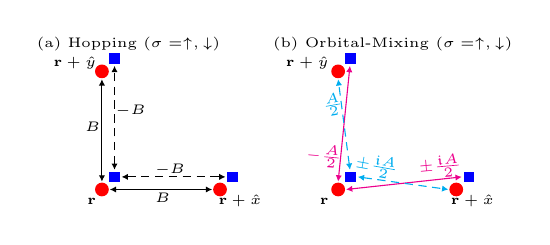
\begin{tikzpicture}

\draw[{Latex[length=0.8mm,width=0.8mm]}-{Latex[length=0.8mm,width=0.8mm]}] (0.05,-0.05)to (1.35,-0.05);
\draw[{Latex[length=0.8mm,width=0.8mm]}-{Latex[length=0.8mm,width=0.8mm]}] (-0.05,0.05)to (-0.05,1.35);

\draw[{Latex[length=0.8mm,width=0.8mm]}-{Latex[length=0.8mm,width=0.8mm]},densely dashed] (0.2,0.11)to (1.52,0.11);
\draw[{Latex[length=0.8mm,width=0.8mm]}-{Latex[length=0.8mm,width=0.8mm]},densely dashed] (0.11,0.2)to (0.11,1.52);


\node [right,black] at (0.5,0.2) {\tiny{$-B$}};
\node [right,black] at (0.5,-0.15) {\tiny{$B$}};

\node [right,black] at (-0.0,0.95) {\tiny{$-B$}};
\node [left,black] at (0.05,0.75) {\tiny{$B$}};

\filldraw[fill=red, draw=red](-0.05,-0.05) circle (0.8mm);
\filldraw[fill=blue, draw=blue](0.05,0.05) rectangle (0.17,0.17);

\filldraw[fill=red, draw=red](-0.05,1.45) circle (0.8mm);
\filldraw[fill=blue, draw=blue](0.05,1.55) rectangle (0.17,1.67);
\filldraw[fill=red, draw=red](1.45,-0.05) circle (0.8mm);
\filldraw[fill=blue, draw=blue](1.55,0.05) rectangle (1.67,0.17);

\draw[{Latex[length=0.8mm,width=0.8mm]}-{Latex[length=0.8mm,width=0.8mm]},magenta] (3.05,-0.05)to (4.52,0.11);
\draw[{Latex[length=0.8mm,width=0.8mm]}-{Latex[length=0.8mm,width=0.8mm]},magenta] (2.95,0.05)to (3.1,1.52);

\draw[{Latex[length=0.8mm,width=0.8mm]}-{Latex[length=0.8mm,width=0.8mm]},cyan,densely dashed] (3.2,0.11)to (4.35,-0.05);
\draw[{Latex[length=0.8mm,width=0.8mm]}-{Latex[length=0.8mm,width=0.8mm]},cyan,densely dashed] (3.1,0.2)to (2.95,1.35);

\node [right,magenta,rotate=5] at (3.85,0.21) {\tiny{$\pm\frac{\mathfrak{i}A}{2}$}};
\node [right,cyan,rotate=-10] at (3.05,0.315) {\tiny{$\pm\frac{\mathfrak{i}A}{2}$}};

\node [right,magenta,rotate=-5] at (2.42,0.4) {\tiny{$-\frac{A}{2}$}};
\node [right,cyan,rotate=10] at (2.63,0.98) {\tiny{$\frac{A}{2}$}};


\filldraw[fill=red, draw=red](2.95,-0.05) circle (0.8mm);
\filldraw[fill=blue, draw=blue](3.05,0.05) rectangle (3.17,0.17);

\filldraw[fill=red, draw=red](2.95,1.45) circle (0.8mm);
\filldraw[fill=blue, draw=blue](3.05,1.55) rectangle (3.17,1.67);
\filldraw[fill=red, draw=red](4.45,-0.05) circle (0.8mm);
\filldraw[fill=blue, draw=blue](4.55,0.05) rectangle (4.67,0.17);

\node [left,black] at (2.95,-0.2) {\tiny{$\mathbf{r}$}};
\node [left,black] at (5.05,-0.2) {\tiny{$\mathbf{r}+\hat{x}$}};
\node [left,black] at (2.95,1.55) {\tiny{$\mathbf{r}+\hat{y}$}};

\node [left,black] at (0.0,-0.2) {\tiny{$\mathbf{r}$}};
\node [left,black] at (2.1,-0.2) {\tiny{$\mathbf{r}+\hat{x}$}};
\node [left,black] at (0.0,1.55) {\tiny{$\mathbf{r}+\hat{y}$}};



\node [right,black] at (-1,1.8) {\tiny{(a) Hopping ($\sigma=\uparrow,\downarrow$)}};
\node [right,black] at (2,1.8) {\tiny{(b) Orbital-Mixing ($\sigma=\uparrow,\downarrow$)}};



\end{tikzpicture}
\end{document}

%Hopping
%\draw[{Latex[length=0.8mm,width=0.8mm]}-{Latex[length=0.8mm,width=0.8mm]},magenta] (0.05,-0.1)to [bend right,looseness=1.3,out=-30,in=210](1.35,-0.1);

%\draw[{Latex[length=0.8mm,width=0.8mm]}-{Latex[length=0.8mm,width=0.8mm]},magenta] (-0.1,0.05)to [bend left,looseness=1.3,out=30,in=-210](-0.1,1.35);

%\draw[{Latex[length=0.8mm,width=0.8mm]}-{Latex[length=0.8mm,width=0.8mm]},magenta,densely dashed] (0.2,0.16)to [bend right,looseness=1.3,out=30,in=-210](1.52,0.16);

%\draw[{Latex[length=0.8mm,width=0.8mm]}-{Latex[length=0.8mm,width=0.8mm]},magenta,densely dashed] (0.16,0.2)to [bend right,looseness=1.3,out=-30,in=210](0.16,1.52);




%Orbital Mixing
%\draw[{Latex[length=0.8mm,width=0.8mm]}-{Latex[length=0.8mm,width=0.8mm]},cyan] (3.05,-0.1)to [bend right,looseness=1.3,out=-30,in=210](4.35,-0.1);

%\draw[{Latex[length=0.8mm,width=0.8mm]}-{Latex[length=0.8mm,width=0.8mm]},cyan] (2.9,0.05)to [bend left,looseness=1.3,out=30,in=-210](2.9,1.35);

%\draw[{Latex[length=0.8mm,width=0.8mm]}-{Latex[length=0.8mm,width=0.8mm]},cyan,densely dashed] (3.2,0.16)to [bend right,looseness=1.3,out=30,in=-210](4.52,0.16);

%\draw[{Latex[length=0.8mm,width=0.8mm]}-{Latex[length=0.8mm,width=0.8mm]},cyan,densely dashed] (3.16,0.2)to [bend right,looseness=1.3,out=-30,in=210](3.16,1.52);
